
% Template of basic phisics experiment 基于 article template, 在此基础上做修改
% 设定文章编码类型, 正文字号为五号则 zihao=5, 正文字号为小四则 zihao=-4
\documentclass[zihao=5, UTF8]{article}		


% 自定义宏定义
\def\N{\mathbb{N}}
\def\F{\mathbb{F}}
\def\Z{\mathbb{Z}}
\def\Q{\mathbb{Q}}
\def\R{\mathbb{R}}
\def\C{\mathbb{C}}
\def\T{\mathbb{T}}
\def\S{\mathbb{S}}
\def\A{\mathbb{A}}
\def\I{\mathscr{I}}
\def\d{\mathrm{d}}
\def\p{\partial}


% 物理实验报告所需的其它宏包
\usepackage{ulem}   % \uline 下划线支持

% 导入基本宏包
\usepackage[UTF8]{ctex}     % 设置文档为中文语言
\usepackage[colorlinks, linkcolor=blue, anchorcolor=blue, citecolor=blue, urlcolor=blue]{hyperref}  % 宏包: 自动生成超链接 (此宏包与标题中的数学环境冲突)
% \usepackage{docmute}    % 宏包: 子文件导入时自动去除导言区, 用于主/子文件的写作方式, \include{./51单片机笔记}即可. 注: 启用此宏包会导致.tex文件capacity受限. 
\usepackage{amsmath}    % 宏包: 数学公式
\usepackage{mathrsfs}   % 宏包: 提供更多数学符号
\usepackage{amssymb}    % 宏包: 提供更多数学符号
\usepackage{pifont}     % 宏包: 提供了特殊符号和字体
\usepackage{extarrows}  % 宏包: 更多箭头符号

% 列表环境设置
\usepackage{enumitem}   % 宏包: 列表环境设置
    \setlist[enumerate]{itemsep=0pt, parsep=0pt, topsep=0pt, partopsep=0pt, leftmargin=3.5em} 
    \setlist[itemize]{itemsep=0pt, parsep=0pt, topsep=0pt, partopsep=0pt, leftmargin=3.5em}
    \newlist{circledenum}{enumerate}{1} % 创建一个新的枚举环境  
    \setlist[circledenum,1]{  
        label=\protect\circled{\arabic*}, % 使用 \arabic* 来获取当前枚举计数器的值, 并用 \circled 包装它  
        ref=\arabic*, % 如果需要引用列表项, 这将决定引用格式（这里仍然使用数字）
        itemsep=0pt, parsep=0pt, topsep=0pt, partopsep=0pt, leftmargin=3.5em
    }  
% 文章页面 margin 设置
\usepackage[a4paper]{geometry}  % 宏包: 文章页面 margin 设置
    \geometry{top=0.75in}
    \geometry{bottom=0.75in}
    \geometry{left=0.75in}
    \geometry{right=0.75in}   % 设置上下左右页边距
    \geometry{marginparwidth=1.75cm}    % 设置边注距离（注释、标记等）

% 自定义数学环境
\usepackage{amsthm} % 宏包: 数学环境配置
% theorem-line 环境自定义
    \newtheoremstyle{MyLineTheoremStyle}% <name>
        {11pt}% <space above>
        {11pt}% <space below>
        {}% <body font> 使用默认正文字体
        {}% <indent amount>
        {\bfseries}% <theorem head font> 设置标题项为加粗
        {: }% <punctuation after theorem head>
        {.5em}% <space after theorem head>
        {\textbf{#1}\thmnumber{#2}\ \ (\,\textbf{#3}\,)}% 设置标题内容顺序
    \theoremstyle{MyLineTheoremStyle} % 应用自定义的定理样式
    \newtheorem{LineTheorem}{Theorem.\,}
% theorem-block 环境自定义
    \newtheoremstyle{MyBlockTheoremStyle}% <name>
        {11pt}% <space above>
        {11pt}% <space below>
        {}% <body font> 使用默认正文字体
        {}% <indent amount>
        {\bfseries}% <theorem head font> 设置标题项为加粗
        {: \\ \indent}% <punctuation after theorem head>
        {.5em}% <space after theorem head>
        {\textbf{#1}\thmnumber{#2}\ \ (\,\textbf{#3}\,)}% 设置标题内容顺序
    \theoremstyle{MyBlockTheoremStyle} % 应用自定义的定理样式
    \newtheorem{BlockTheorem}[LineTheorem]{Theorem.\,} % 使用 LineTheorem 的计数器
% definition 环境自定义
    \newtheoremstyle{MySubsubsectionStyle}% <name>
        {11pt}% <space above>
        {11pt}% <space below>
        {}% <body font> 使用默认正文字体
        {}% <indent amount>
        {\bfseries}% <theorem head font> 设置标题项为加粗
        {: \\ \indent}% <punctuation after theorem head>
        {0pt}% <space after theorem head>
        {\textbf{#3}}% 设置标题内容顺序
    \theoremstyle{MySubsubsectionStyle} % 应用自定义的定理样式
    \newtheorem{definition}{}


% 有色文本框及其设置
\usepackage[dvipsnames,svgnames]{xcolor}    %设置插入的文本框颜色
\usepackage[strict]{changepage}     % 提供一个 adjustwidth 环境
\usepackage{framed}     % 实现方框效果
    \definecolor{graybox_color}{rgb}{0.95,0.95,0.96} % 文本框颜色. 修改此行中的 rgb 数值即可改变方框纹颜色, 具体颜色的rgb数值可以在网站https://colordrop.io/ 中获得. （截止目前的尝试还没有成功过, 感觉单位不一样）（找到喜欢的颜色, 点击下方的小眼睛, 找到rgb值, 复制修改即可）
    \newenvironment{graybox}{%
    \def\FrameCommand{%
    \hspace{1pt}%
    {\color{gray}\small \vrule width 2pt}%
    {\color{graybox_color}\vrule width 4pt}%
    \colorbox{graybox_color}%
    }%
    \MakeFramed{\advance\hsize-\width\FrameRestore}%
    \noindent\hspace{-4.55pt}% disable indenting first paragraph
    \begin{adjustwidth}{}{7pt}%
    \vspace{2pt}\vspace{2pt}%
    }
    {%
    \vspace{2pt}\end{adjustwidth}\endMakeFramed%
    }

% 各级标题自定义设置
\usepackage{titlesec}   
    % section标题自定义设置 
    \titleformat{\section}[hang]{\normalfont\huge\bfseries\centering}{第\,\thesection\,部分}{20pt}{}
    % subsection标题自定义设置 
    \titleformat{\subsection}[hang]{\normalfont\Large\bfseries}{\,\thesubsection\,}{8pt}{}
    % subsubsection标题自定义设置
    \titleformat{\subsubsection}[hang]{\normalfont\large\bfseries}{\,\thesubsubsection\,}{6pt}{}

% 外源代码插入设置
\usepackage{matlab-prettifier}
    \lstset{
        style=Matlab-editor,  % 继承matlab代码颜色等
    }
\usepackage[most]{tcolorbox} % 引入tcolorbox包 
\usepackage{listings} % 引入listings包
    \tcbuselibrary{listings, skins, breakable}
    \lstdefinestyle{matlabstyle}{
        language=Matlab,
        basicstyle=\small,
        breakatwhitespace=false,
        breaklines=true,
        captionpos=b,
        keepspaces=true,
        numbers=left,
        numbersep=15pt,
        showspaces=false,
        showstringspaces=false,
        showtabs=false,
        tabsize=2
    }
    \newtcblisting{matlablisting}{
        arc=0pt,
        top=0pt,
        bottom=0pt,
        left=1mm,
        listing only,
        listing style=matlabstyle,
        breakable,
        colback=white   % 选一个合适的颜色
    }

% table 支持
\usepackage{booktabs}   % 宏包: 三线表
\usepackage{tabularray} % 宏包: 表格排版
\usepackage{longtable}  % 宏包: 长表格

% figure 设置
\usepackage{graphicx}  % 支持 jpg, png, eps, pdf 图片 
\usepackage{svg}       % 支持 svg 图片
    \svgsetup{
        % 指向 inkscape.exe 的路径
        inkscapeexe = C:/aa_MySame/inkscape/bin/inkscape.exe, 
        % 一定程度上修复导入后图片文字溢出几何图形的问题
        inkscapelatex = false                 
    }


% 图表进阶设置
\usepackage{float}     % 图表位置浮动设置 
\usepackage{caption}    % 图注、表注
    \captionsetup[figure]{name=图}  
    \captionsetup[table]{name=表}
    \captionsetup{labelfont=bf, font=small}

% 文章默认字体设置
    \usepackage{fontspec}   % 宏包: 字体设置
        \setmainfont{SimSun}[
            BoldFont = SimHei, % 设置粗体字为黑体
            ItalicFont = KaiTi, % 设置斜体字为楷体
            BoldItalicFont = KaiTi % 设置粗斜体字为楷体
        ] 
        %\setCJKmainfont[AutoFakeBold=3]{SimSun} % 设置加粗字体为 SimSun 族, AutoFakeBold 可以调整字体粗细
        \setmainfont{Times New Roman} % 设置英文字体为Times New Roman


% 其它设置
    % equation 公式编号设置
        \makeatletter  
        \renewcommand{\theequation}{\thesection.\arabic{equation}}  
        \makeatother
    % 脚注设置
        \renewcommand\thefootnote{\ding{\numexpr171+\value{footnote}}}
    % 参考文献引用设置
        \bibliographystyle{unsrt}   % 设置参考文献引用格式为unsrt
        \newcommand{\upcite}[1]{\textsuperscript{\cite{#1}}}     % 自定义上角标式引用
    % 文章序言设置
        \newcommand{\cnabstractname}{序言}
        \newenvironment{cnabstract}{%
            \par\Large
            \noindent\mbox{}\hfill{\bfseries \cnabstractname}\hfill\mbox{}\par
            \vskip 2.5ex
            }{\par\vskip 2.5ex}


% 页眉页脚设置
\usepackage{fancyhdr}   %宏包: 页眉页脚设置
    \pagestyle{fancy}
    \fancyhf{}
    \cfoot{\thepage}
    \renewcommand\headrulewidth{1pt}
    \renewcommand\footrulewidth{0pt}
    \rhead{\bfseries 分组序号: 3-04-1}    
    \chead{《基础物理实验》实验报告,\ 潘天麟\ 2023K8009908023}
    \lhead{2024.10.23}

% 开始编辑文章

\begin{document}
\noindent\begin{flushright}
    \zihao{2}{分组序号: 3-04-1}
\end{flushright}

\setCJKfamilyfont{boldsong}[AutoFakeBold = {2.17}]{SimSun}
\newcommand*{\boldsong}{\CJKfamily{boldsong}}


\begin{center}\large
    \noindent{\Huge\bfseries\boldsong《基础物理实验》实验报告 }
    \\\vspace{0.4cm}
    \noindent\textit{
        \textbf{\boldsong 实验名称: }\uline{\hspace{2.3cm} 傅里叶光学基础\hspace{2.3cm}}\hspace{0.4cm} 
        指导教师: \uline{\hspace{1.5cm}李运良\hspace{1.5cm}}}
    \\\vspace{0.1cm}
    \noindent\textit{
        姓名: \uline{\,\,潘天麟\,\,}\hspace{0.2cm}
        学号: \uline{\,\,{\upshape 2023K8009908023}\,\,}\hspace{0.2cm}
        专业: \uline{\,\,人工智能\,\,}\hspace{0.2cm}
        班级: \uline{\,\,\upshape{2313}\,\,}\,组号: \uline{\,\,\upshape{3-04-1}\,\,}}
    \\\vspace{0.1cm}
    \noindent\textit{
        实验日期: \uline{\,\,{\upshape 2024.10.23}\,\,}\hspace{0.2cm}
        实验地点: \uline{\,\,\,教学楼{\upshape705}\,\,\,}\hspace{0.2cm}
        是否调课/补课: \uline{\hspace{1.3cm}}\hspace{0.2cm}
        成绩: \uline{\hspace{2cm}}}
\end{center}
% \vspace{-0.2cm}
\noindent\rule{\textwidth}{0.1em}   % 分割线
\section{实验目的}

\subsection{阿贝成像与基本空间滤波}
\begin{enumerate}
    \item 掌握一维导轨上光路的调节. 
    \item 通过搭建阿贝成像光路和观察不同空间滤波器的效果, 体会和理解成像过程、频谱面、谱空间与实空间对应关系、空间滤波、衍射等物理概念. 
\end{enumerate}

\subsection{光学4F系统成像}
体会和掌握光学4F成像系统的组织和搭建；在前面阿贝成像实验的基础上, 进一步体会更为复杂的光学信息处理. 光学4F系统目前广泛应用于飞秒激光脉冲整形器中, 产生不同频带和脉宽的光脉冲. 

\subsection{假彩色编码}
在基本空间滤波的基础上, 进一步体会光栅衍射的色散效果和选频滤波操作, 掌握$\theta$调制假彩色编码的选频滤波和色散选区滤波的原理；并利用提前预制分区信息的光栅图案, 实现该图像的假彩色编码. 

\subsection{光栅光谱仪实验}
\subsubsection{夫琅和费衍射演示实验}
将分划板放入光路中,看衍射图样的变化,根据所学判断衍射图样与分划板参数是否一致. 
\subsubsection{光栅衍射测量光栅常量实验}
将透射光栅放入光路中, 看衍射光斑图样, 根据光栅方程算出光栅常数 \(d\), 判断与已知光栅刻缝数是否一致. 

\subsubsection{光栅光谱仪测光谱实验}
使用手持式光栅光谱仪和 SpectraSmart 软件测量白光或单色光光谱,记录中心波长、峰值强度与线宽,判断与经验值是否一致. 


\section{实验仪器}

\subsection{阿贝成像与基本空间滤波激光器组件}
\begin{itemize}
    \item 激光器组件: 激光器、棱镜夹持器、一维平移台、宽滑块、支杆和套筒
    \item 扩束镜组件: 凹透镜（$\Phi 6$, $f=-10\text{mm}$）、透镜架、滑块、支杆和套筒
    \item 准直镜组件: 凸透镜（$\Phi 40$, $f=80\text{mm}$）、透镜架、滑块、支杆和套筒
    \item 光栅字组件: 光栅字（$\Phi 40$, 10 线/mm）、滑块、支杆和套筒
    \item 变换透镜组件: 凸透镜（$\Phi 76$, $f=175\text{mm}$）、镜架、滑块、支杆和套筒
    \item 滤波器组件: 滤波器（低通、方向滤波）、干板架、滑块、支杆和套筒
    \item 白屏组件: 白屏、干板架、滑块、支杆和套筒
\end{itemize}

\subsection{光学4F系统成像}
\begin{itemize}
    \item 光源组件: 半导体激光器（650nm）、一维平移台、宽滑块、支杆和套筒
    \item 准直镜组件: 凹透镜（$\Phi 6$, $f=-9.8\text{mm}$）、凸透镜（$\Phi 25$, $f=80\text{mm}$）、透镜架、滑块、支杆和套筒
    \item 制物组件: 物板、干板架、滑块、支杆和套筒
    \item 变换透镜组件: 凸透镜（$\Phi 40$, $f=150\text{mm}$）2 个、镜架、滑块、支杆和套筒
    \item 滤波器组件: 滤波器（低通、方向滤波）、精密平移台、干板夹、滑块、支杆和套筒
    \item 屏组件: 白屏、干板架、滑块、支杆和套筒
\end{itemize}

\subsection{假彩色编码}
\begin{itemize}
    \item 光源组件: 白光 LED、一维平移台、宽滑块、支杆和套筒
    \item 准直镜组件: 凸透镜（$\Phi 40$, $f=80\text{mm}$）、透镜架、滑块、支杆和套筒
    \item 调制物组件: 天安门光栅（100 线/mm）、干板架、滑块、支杆和套筒
    \item 变换透镜组件: 凸透镜（$\Phi 76$, $f=175\text{mm}$）、镜架、滑块、支杆和套筒
    \item 滤波器组件: 滤波器、干板架、滑块、支杆和套筒
    \item 白屏组件: 白屏、干板架、滑块、支杆和套筒
\end{itemize}

\subsection{光栅光谱仪实验}
\begin{itemize}
    \item 光源组件: 半导体激光器（650nm）、一维平移台、宽滑块、支杆和套筒
    \item 滤波器组件: 滤波器、干板架、滑块、支杆和套筒
    \item 白屏组件: 白屏、干板架、滑块、支杆和套筒
    \item 透射光栅, 手持式光栅光谱仪
    \item 分划板, 参数如下
\end{itemize}



\begin{figure}[H]
    \centering
    \begin{minipage}[t]{0.45\textwidth}
        \centering
        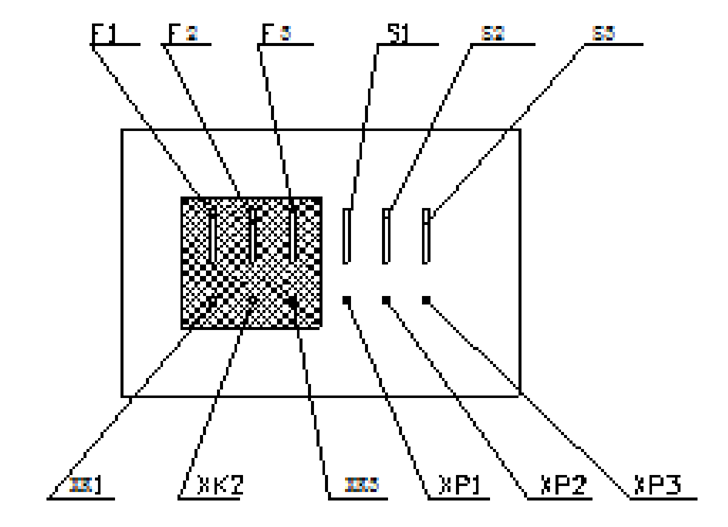
\includegraphics[width=0.6\linewidth]{imgs/分划板1.png} 
        \caption{分划板1}
    \end{minipage}%
    \begin{minipage}[t]{0.45\textwidth}
        \centering
        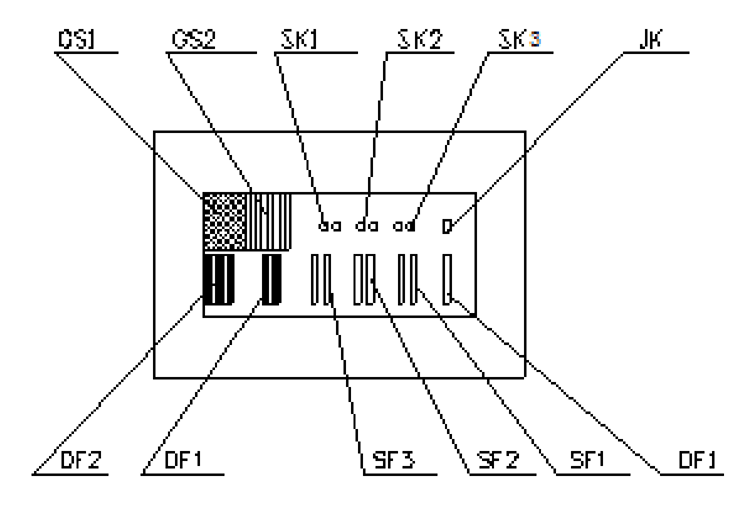
\includegraphics[width=0.6\linewidth]{imgs/分划板2.png} 
        \caption{分划板2}
    \end{minipage}
\end{figure}

\begin{figure}[H]
    \centering
    \begin{minipage}[t]{0.45\textwidth}
        \centering
        \begin{tabular}{@{}ll@{}}
        \toprule
        \textbf{类型} & \textbf{参数} \\
        \midrule
        单缝 & F1: \(a=0.1\) \\
            & F2: \(a=0.2\) \\
            & F3: \(a=0.3\) \\
        单丝 & S1: \(a=0.1\) \\
            & S2: \(a=0.2\) \\
            & S3: \(a=0.3\) \\
        小孔 & XK1: \(\phi=0.2\) \\
            & XK2: \(\phi=0.3\) \\
            & XK3: \(\phi=0.4\) \\
        小屏 & XP1: \(\phi=0.2\) \\
            & XP2: \(\phi=0.3\) \\
            & XP3: \(\phi=0.4\) \\
        \bottomrule
        \end{tabular}
        \captionof{table}{分划板1参数}
    \end{minipage}%
    \begin{minipage}[t]{0.45\textwidth}
        \centering

        \begin{tabular}{@{}ll@{}}
        \toprule
        \textbf{类型} & \textbf{参数} \\
        \midrule
        光栅 & GS1: 纵横均为 50 条/mm \\
            & GS2: 纵向 50 条/mm \\
        双孔 & SK1: \(d=0.25\), \(\phi=0.2\) \\
            & SK2: \(d=0.32\) \\
            & SK3: \(d=0.4\) \\
        矩孔 & JK: \(a=0.12, b=0.2\) \\
        单缝 & DF1: \(a=0.08\) (右下 1) \\
        双缝 & SF1: \(a=0.08, d=0.16\) \\
            & SF2: \(a=0.08, d=0.20\) \\
            & SF3: \(a=0.06, d=0.10\) \\
        多缝 & DF1: 4 缝 \(a=0.06, d=0.1 \times 4\) \\
            & DF2: 9 缝 \(a=0.06, d=0.1 \times 9\) \\
        \bottomrule
        \end{tabular}

        \captionof{table}{分划板2参数}
    \end{minipage}
\end{figure}
\section{实验原理}

\subsection{阿贝成像与基本空间滤波}

\subsubsection{阿贝成像原理}

\begin{enumerate}
    \item 入射光场被物平面衍射形成一个携带物信息的衍射场, 该衍射场经过透镜的变换操作在频谱面形成频谱斑, 而这些衍射斑就是“物”信息与光场卷积后的变换花样. 
    \item 这些携带了“物”信息的频谱斑成为新的相干光源发射球面波, 并通过光场的进一步传播在像平面实现退卷积, 从而干涉成像. 
\end{enumerate}

\subsubsection{阿贝成像原理的证明和思路}

\begin{enumerate}
    \item 物、透镜、频谱面和像面都在 \(x, y\) 面内, 光场沿 \(z\) 方向传播；透镜焦距为 \(F\), 单色相干光源波长为 \(\lambda\). 
    \item 任何一个物对于一个单色平行入射的相干光源的调整, 可以理解或者转化为一系列沿空间方向变化的余弦光栅的总和；暂时只考虑仅 \(x\) 方向的变化, 因为 \(x, y\) 方向是正交和独立的, 所以 \(y\) 方向可以类比 \(x\) 方向的讨论和结果. 这些不同频率的余弦光栅的空间频率为 \(f_i\), 物光波波前为
    \[
    U_{\text{ob}}(x, y) = A_1(t_0 + t_i \cos(2\pi f_i x)).
    \]
    \item 仅考虑其中一个单频信息 \(f_i\), 其经过物镜变换后, 该光场会在后焦面即频谱面形成三个点状衍射斑 \(S_0, S_{+1}\) 和 \(S_{-1}\)；这三个点状衍射斑中, \(S_0\) 处于 \(xy\) 平面的中心, 即 \(S_0 = 0\)；而 \(S_{+1}\) 和 \(S_{-1}\) 分别对称地分布在 \(x\) 方向的偏轴位置上, 其偏轴距离满足
    \[
    S_{\pm 1} = \pm F \tan \theta_i, \quad \text{其中} \quad \sin \theta_i = f_i \lambda.
    \]
    这三个相干点光源成为新的次级光源, 然后发射球面波；这三个点源的光场复振幅分别为
    \[
    A_0 \propto A_1 t_0 e^{ik L(B S_0)}, \quad A_{+1} \propto A_1 t_i e^{ik L(B S_{+1})}/2, \quad A_{-1} \propto A_1 t_i e^{ik L(B S_{-1})}/2.
    \]
    这三个新光源的相干光在像面形成干涉, 其干涉像场最终结果为
    \[
    U_{\text{im}}(x', y') = K e^{ik \frac{x'^2 + y'^2}{2z}} A_1(t_0 + t_i \cos(2\pi f_i' x')).
    \]
\end{enumerate}

根据以上讨论, 我们可以得到: 
\begin{enumerate}
    \item 物原本的单频信息 \(f_i\) 可以在像面重构为相似的但是空间频率为 \(f_i'\) 的信号, 其比值就是放大率 \(V \equiv \frac{f_i'}{f_i}\)；
    \item 考虑到一个一般性的物是一系列 \(f_i\) 的组合, 因此在像面也会成一个同样的由 \(f_i'\) 组合的像, 其放大率为 \(V\)；
    \item 频谱面上的 \(S_0\) 对应的就是物信息中的 0 频信息 \(A_1 t_0\), 其位置处于面内的源点；正负两方向的衍射点 \(S_{+1}\) 和 \(S_{-1}\) 代表了指定频率 \(f_i'\) 的信息 \(A_1 t_i\), 其位置由焦距 \(F\) 和衍射角 \(\theta_i\) 决定, 空间频率 \(f_i\) 越大, 衍射角 \(\theta_i\) 就越高, 衍射点 \(S_{+1}\) 和 \(S_{-1}\) 离中心就越远. 
\end{enumerate}

\subsection{光学 4F 系统成像}

一束平行光照射透明物体（待处理的图像）, 物置于第一个透镜的前焦面处. 在第一透镜的后焦面上得到物函数 \(g(x_0, y_0)\) 的频谱 \(G(f_\xi, f_\eta)\). 此频谱面又位于第二透镜的前焦面上, 在第二透镜的后焦面上得到频谱函数的傅里叶变换 \(g(x, y)\). 物函数经过两次傅里叶变换又得到了原函数, 只是变成了倒像. 

\subsection{假彩色编码}

一个白光光源照射透明的天安门（物面上的被调制物）, 然后携带了物信息的衍射场会继续向前传播. 这时由于入射光为白光且光栅的衍射行为, 不同颜色的光会分散开了, 开始呈现多彩颜色. 衍射场经透镜重新汇聚, 在频谱面会形成较清晰的彩色频谱花样. 由于天安门花样上不同的区域（天空、天安门、草地）的光栅方向是不同的, 所以其衍射花样也会延三个不同方向展开, 呈现出彩色的带状花样. 

\section{实验步骤}
\begin{figure}[H]
    \centering
    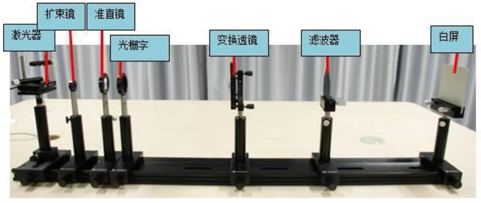
\includegraphics[width=0.8\textwidth]{imgs/实验步骤图1.png}
    \caption{阿贝成像与基本空间滤波实验光路}
\end{figure}
\subsection{阿贝成像与基本空间滤波}
\begin{enumerate}
    \item 光路布置调节
    \begin{enumerate}
        \item 参照图 1 布置光路, 自左向右依次为激光器组件、扩束镜组件、准直镜组件、光栅字组件、变换透镜组件、滤波器组件和白屏组件. （相邻组件纵向间隔距离参考数值, 即图 3 中红线与红线之间距离依次 40mm、70mm、40mm、240mm、195mm 和 445mm）. 
        \item 等高平行: 安装激光器和白屏, 调整激光器出光口到支杆顶部距离为 90mm（仅供参考）, 调试平移台及激光器俯仰使其沿导轨中心水平传播. 调试之前可选择固定参考高度（比如在白屏中心上刻度）, 反复调节白屏前后位置, 直到激光在近处和远处均能打在白屏上同样参考高度位置, 则视为激光器水平调整完成. 
        \item 安装扩束镜, 上下调整支杆使扩束光斑中心与参考中心重合, 然后固定. 
        \item 安装准直镜, 准直镜距扩束镜大概 70mm（共焦调整）即可获得平行光, 上下调整支杆使平行光束与参考中心重合, 然后固定. 
        \item 安装光栅字, 上下调整支杆使光斑正入射"光"字, 然后固定. 光栅字位置尽可能靠近准直镜. 
        \item 安装变换透镜, 上下调整支杆使入射"光"字从变换透镜中心通过, 此时在白屏上可看到模糊像, 前后移动变换透镜直至在白屏上看到清晰的放大倒立实像, 然后固定. 
        \item 安装滤波器, 沿导轨前后移动滤波器, 同时观察滤波器上的花样；当花样最清晰时, 即为变换透镜的频谱面位置, 应在此处固定滤波器支架. 
        \item 测试不同滤波器: 在后面的实验中, 在滤波器支架上使用不同的滤波器, 观察屏上的滤波后的效果. 注意在此过程中, 不要移动所有的光学器件的位置, 包括滤波器支架的水平位置. 
    \end{enumerate}
    \item 观察"光"栅字的像和频谱
    去掉滤波器, 观察没有滤波状态下的物像, 当放大倍数足够大时（像距足够远时）, 我们应该可以观察到"光"字的像中间既有横向条纹, 也有竖向条纹. 
    实验中使用的"光"字是用空间频率为12 线/mm的正交光栅调制的, 在变换透镜的频谱面上放置一个屏, 即可观察到频谱点, 可根据目标物分析频谱. 
    \item 观察方向滤波和低通滤波的实际效果
    \begin{enumerate}
        \item 选择滤波器中的"缝", 在频谱面水平放置, 使包括 0 级在内的一排点通过, 我们可以观察到"光"的像中间充满竖向条纹. 
        \item 将"缝"旋转 90 度竖直放置, 使包括 0 级在内的一排点通过, 我们可以观察到"光"的像中间充满横向条纹. 
        \item 将"缝"旋转 45 度竖直放置, 使包括 0 级在内的一排点通过, 我们可以观察到"光"的像中间充满斜条纹. 
        \item 将滤波器中的"孔"放置在频谱面, 只让 0 级点通过, 我们即可以观察到"光"的像中间没有条纹, 只剩下"光"字轮廓. 
    \end{enumerate}
\end{enumerate}
\subsection{光学4F系统成像}
\begin{enumerate}
    \item 在实验一阿贝成像基础上, 激光器、扩束镜、准直镜和白屏不用移动. 
    \item 安装物孔: 把实验提供的物孔（此处光栅字和带字白纸）垂直方向安装到一个支架上；上下调整支杆使准直后的光斑中心正入射物孔（应使物孔尽可能处于光斑的中心）, 然后固定物孔支杆. 物孔位置应当尽可能靠近准直镜, 以减少不必要的光程；固定物孔支架滑块, 以防移动. 
    \item 安装变换透镜 1: 在物孔后方放置变换透镜 1（f=150mm）, 上下调整支杆使入射物孔后的光, 从变换透镜中心通过, 在此中心位置固定支杆（即固定垂直高度）；然后, 移动变换透镜 1 使其尽可能接近物孔（尽可能减少不必要的光程）, 并在此处固定变换透镜 1 支撑滑块（即固定水平位置）. 
    \item 安装变换透镜 2: 在变换透镜 1 后方放置变换透镜 2 (f=150mm), 上下调整支杆使入射变换透镜1后的光, 从变换透镜2中心通过, 在此中心位置固定支杆（即固定垂直高度）；然后, 移动变换透镜 2 到距离变换透镜 1 两倍焦距的地方, 并在此处固定变换透镜 2 支撑滑块（即固定水平位置）. 注意: 变换透镜是有可能在两个方向上的焦距稍有差异的, 因此两个变换透镜需要对称（或者对易）使用, 即两个变换透镜必须使用相同的焦距方向相对放置. 为了减少像差, 透镜放置原则可以简单记为"凹凸面对准平行光". 
    \item 在白屏上观察成像的特点, 可以看到与物体等大的清晰的物像, 观察与阿贝成像时单透镜成像的区别. 可以在频谱面上安装滤波器, 观察像的变化. 
\end{enumerate}
\subsection{假彩色编码}
\begin{figure}[H]
    \centering
    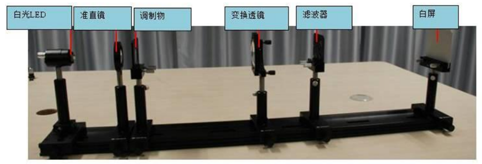
\includegraphics[width=0.8\textwidth]{imgs/实验步骤图2.png}
    \caption{假彩色编码实验光路}
\end{figure}
\begin{enumerate}
    \item 光路布置和调节
    \begin{enumerate}
        \item 按照图 2 布置光路, 自左向右依次为光源组件、准直镜组件、调制物组件、变换透镜组件、滤波器组件和白屏组件. （相邻组件水平方向间隔距离参考数值依次为 40mm、70mm、40mm、240mm、195mm、445mm）. 
        \item 安装白光光源: 安装调整白光 LED 光源；调节 LED 光源支杆高度并固定于支杆靠近中间的位置, 使得 LED 光源到支杆顶端的距离约为 90mm（仅供参考）. 
        \item 安装白屏: 将白屏固定在导轨右侧, 尽量远一些. 
        \item 安装准直镜: 在距离 LED 发光点大约150mm附近放置准直透镜；然后, 首先调节准直透镜的高度, 使得 LED 光源发光点与准直透镜的中心水平对齐, 并在白屏中心, 固定准直透镜的垂直高度；下一步, 水平调节准直透镜的位置, 直到通过其后的白光成为在近处和远处的光斑大小大致一样的准直光. （注意, 由于此处为白光光源, 单透镜有色差, 所以不可能作到绝对的准直；只要在远处的情况下, 最中心的白色亮斑与近处时的白色亮斑大小一致即可. ）在此准直条件下, 固定准直镜支撑滑块（即固定水平位置）. 
        \item 安装天安门光栅: 上下调整支杆使光斑正入射天安门中心, 然后将其固定. 
        \item 安装变换透镜: 上下调整支杆使入射光尽可能从变换透镜中心通过, 此时在白屏上可看到模糊像, 前后移动变换透镜直至在白屏上看到放大倒立实像, 然后固定. 
        \item 安装滤波器: 安装滤波器支架, 并安装一个纸片或者铁片于支架上；然后, 沿导轨水平移动滤波器支架, 并观察衍射光斑的变化；直到纸片或者铁片上呈现清晰的频谱面花样时, 即为变换透镜的频谱面位置；在此处, 固定滤波器支架的水平位置. 后面, 使用不同的滤波器于支架上, 即可实现滤波. 
    \end{enumerate}
    \item $\theta$调制及现象观察
    \begin{enumerate}
        \item 使用$\theta$调制滤波器: 根据预想的各部分图案所需要的颜色, 使用提供的$\theta$调制滤波器（三色滤片滤波器）实现指定的分区着色 – 蓝天、红色天安门、绿地. 首先, 安装$\theta$调制滤波器到滤波器支架上；然后, 调整$\theta$调制滤波器的正反上下左右位置, 使得调制器上的三色滤片与频谱面花样的指定分支相匹配；此处要求, 频谱面花样中的三个衍射方向上, 应当让天安门图案对应的一组衍射谱匹配红色的滤片（即让红色通过）, 草地对应的一组衍射谱条匹配绿色的滤片（即让绿色通过）, 天空对应的一组衍射谱条匹配蓝色的滤片（即让蓝色通过）. 调整好后, 在后面白屏上观看经编码得到的假彩色像. 
    \end{enumerate}
\end{enumerate}

\section{实验数据记录与处理}
\subsection{阿贝成像与基本空间滤波}
\subsubsection{光路布置调节}

\begin{figure}[H]
    \centering
    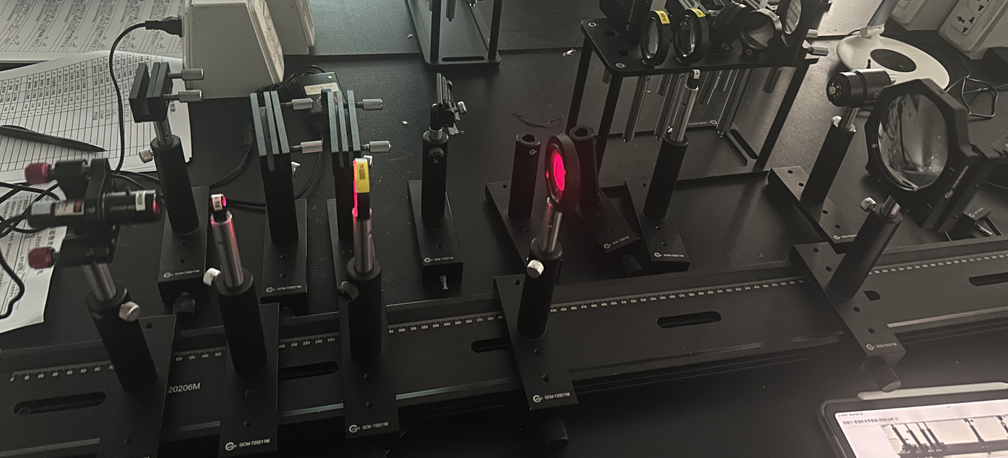
\includegraphics[width=0.6\textwidth]{imgs/实验一光路.png}
    \caption{阿贝成像光路}
\end{figure}

\subsubsection{观察“光”栅字的像和频谱}
观察没有滤波状态下的像和光在频谱面上的频谱如图所示
\begin{figure}[H]
    \centering
    \begin{minipage}[t]{0.45\textwidth}
        \centering
        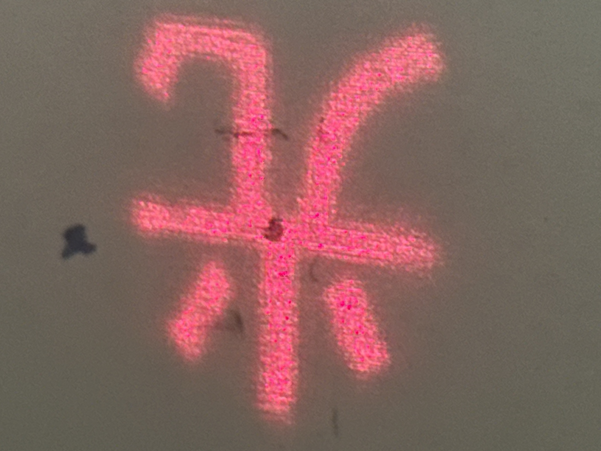
\includegraphics[width=0.8\textwidth]{imgs/光无滤波.png}
        \caption{无滤波状态下的“光”字的像}
    \end{minipage}%
    \begin{minipage}[t]{0.45\textwidth}
        \centering
        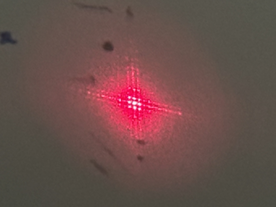
\includegraphics[width=0.8\textwidth]{imgs/光字的频谱.png}
        \caption{“光”字的频谱}
    \end{minipage}%

\end{figure}

加入横向和竖向的滤波器后如图所示
\begin{figure}[H]
    \centering
    \begin{minipage}[t]{0.45\textwidth}
        \centering
        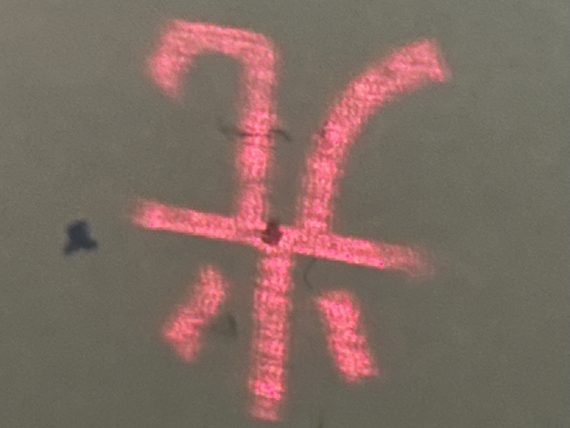
\includegraphics[width=0.8\linewidth]{imgs/光横缝.png} 
        \caption{横向滤波器下的“光”字的像}
    \end{minipage}%
    \begin{minipage}[t]{0.45\textwidth}
        \centering
        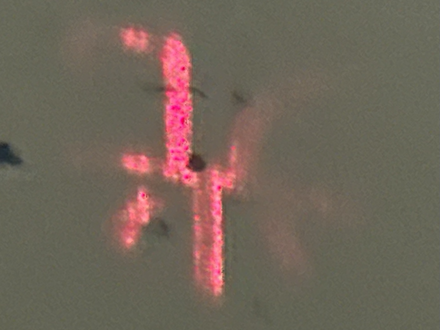
\includegraphics[width=0.8\linewidth]{imgs/光垂缝.png} 
        \caption{竖向滤波器下的“光”字的像}
    \end{minipage}
\end{figure}
可以发现在图中的条纹其实不太明显, 但若放大自己观察, 仍然能够发现在横向滤波器下的像中间充满竖向条纹, 在竖向滤波器下的像中间充满横向条纹. 在实际实验中肉眼的观察效果比拍照要好得多, 这可能是因为相机夜景模式自动长时间曝光使得条纹互相掩盖造成的.
\subsection{光学4F系统成像}
\subsubsection{光路布置调节}

\begin{figure}[H]
    \centering
    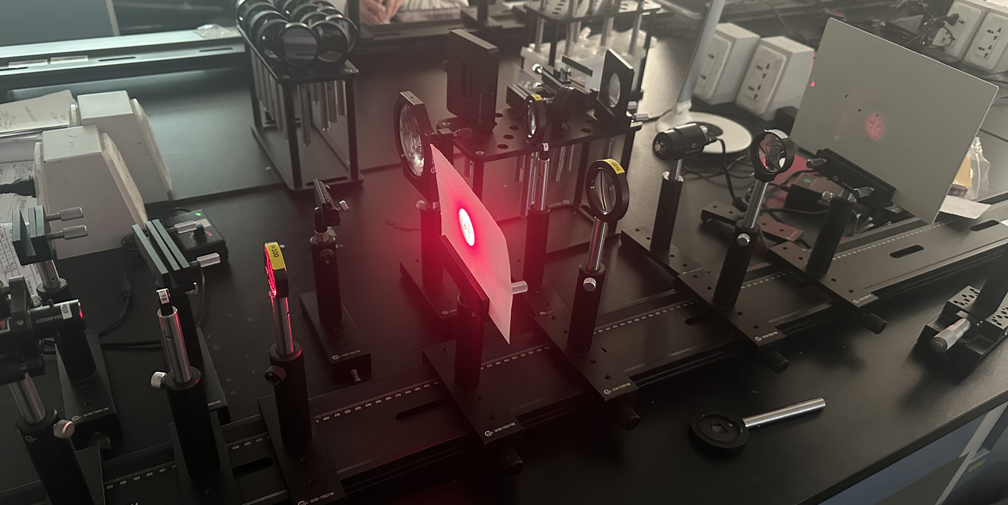
\includegraphics[width=0.6\textwidth]{imgs/实验二光路.png}
    \caption{光学4F系统成像光路}
\end{figure}

\subsubsection{观察成像的特点}
在实验中, 我自己在白纸上绘制了一个“叶”字, 然后观察了其在通过4F系统后的成像效果. 

\begin{figure}[H]
    \centering
    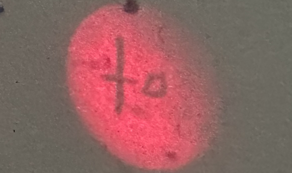
\includegraphics[width=0.6\textwidth]{imgs/叶无滤波.png}
    \caption{“叶”字的像}
\end{figure}
可以看到, 通过4F系统成像后的“叶”字的像是清晰的, 与物体等大, 且是倒立的. 由于滤波实验已经在阿贝成像实验中进行过, 这里就不再重复进行. 

\subsection{假彩色编码}
\subsubsection{光路布置调节}

\begin{figure}[H]
    \centering
    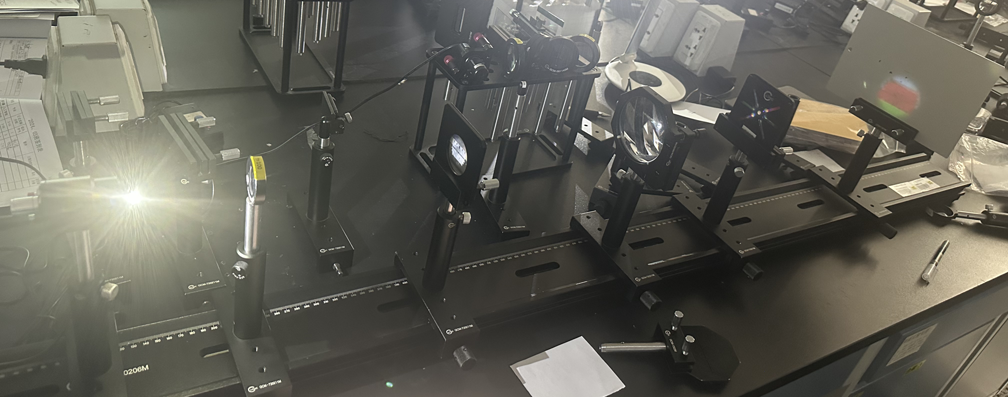
\includegraphics[width=0.6\textwidth]{imgs/实验三光路.png}
    \caption{假彩色编码光路}
\end{figure}
此时可以在频谱面上观察到彩色斑点, 在此处加入$\theta$调制滤波器后, 白屏上可观察到假彩色编码效果

\begin{figure}[H]
    \centering
    \begin{minipage}[t]{0.45\textwidth}
        \centering
        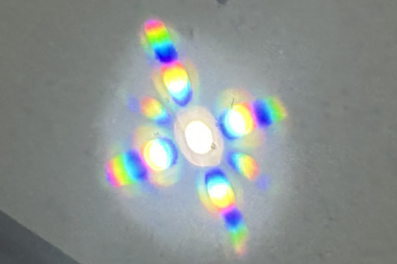
\includegraphics[width=0.8\textwidth]{imgs/天安门频谱.png}
        \caption{天安门的频谱}
    \end{minipage}%
    \begin{minipage}[t]{0.45\textwidth}
        \centering
        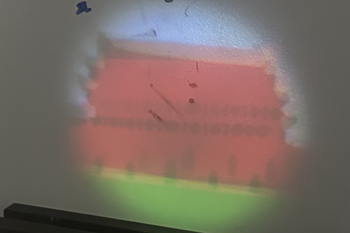
\includegraphics[width=0.8\linewidth]{imgs/天安门.png} 
        \caption{天安门的像}
    \end{minipage}
\end{figure}
可以发现, 通过$\theta$调制滤波器后, 天安门的像被着色, 天空为蓝色, 天安门为红色, 草地为绿色. 

\section{光栅光谱仪实验}
\subsection{夫琅和费衍射演示实验}
\subsubsection{光路布置调节}
\begin{figure}[H]
    \centering
    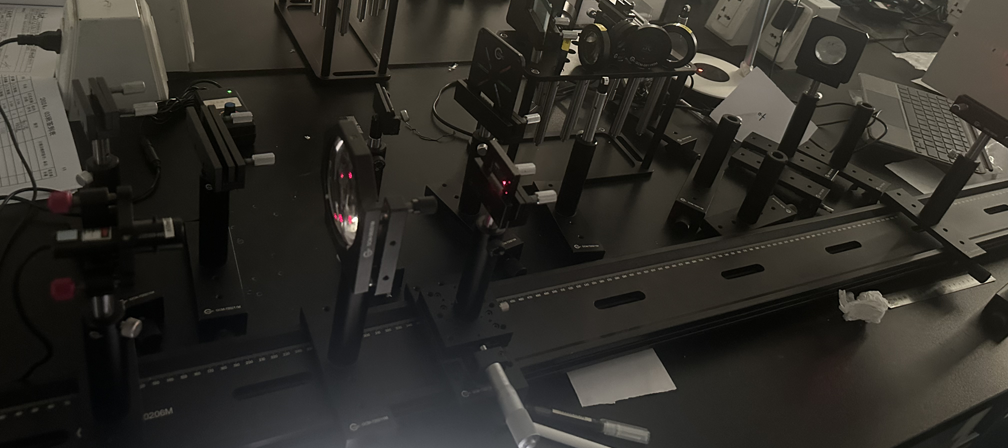
\includegraphics[width=0.6\textwidth]{imgs/分划板光路.png}
    \caption{夫琅和费衍射演示实验光路}
\end{figure}
\subsubsection{观察夫琅和费衍射}
对于分划板1, 我们观察到了如下的衍射图像, 其中各种光栅的参数可参考实验仪器部分的表格. 
\begin{table}[h!]
    \centering
    \begin{tabular}{|ccc|}
        \hline
        \begin{minipage}[t]{0.3\textwidth}
            \centering
            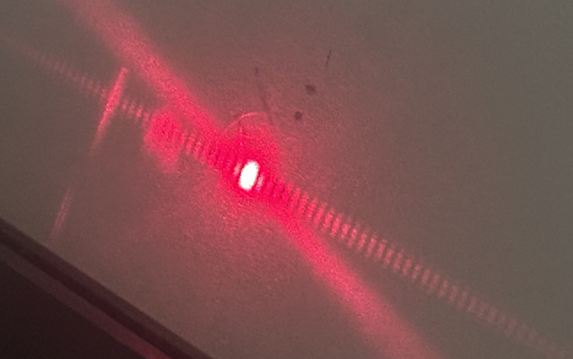
\includegraphics[width=\linewidth]{imgs/f1.png}
            \captionof{figure}{F1}
        \end{minipage} & 
        \begin{minipage}[t]{0.3\textwidth}
            \centering
            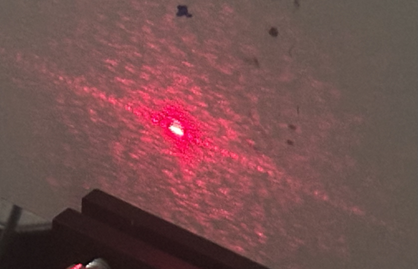
\includegraphics[width=\linewidth]{imgs/f2.png}
            \captionof{figure}{F2}
        \end{minipage} & 
        \begin{minipage}[t]{0.3\textwidth}
            \centering
            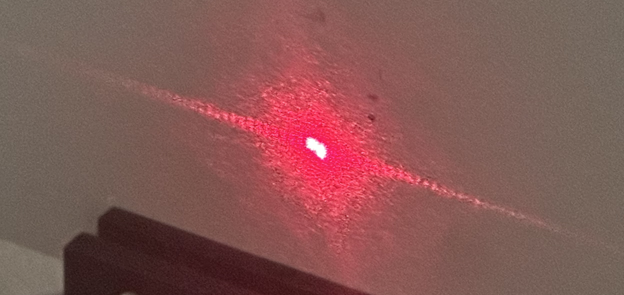
\includegraphics[width=\linewidth]{imgs/f3.png}
            \captionof{figure}{F3}
        \end{minipage} \\
        \begin{minipage}[t]{0.3\textwidth}
            \centering
            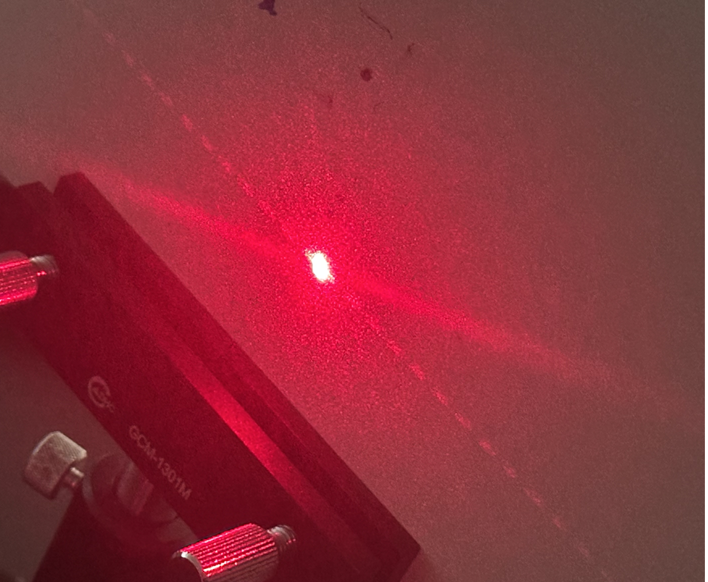
\includegraphics[width=\linewidth]{imgs/s1.png}
            \captionof{figure}{S1}
        \end{minipage} & 
        \begin{minipage}[t]{0.3\textwidth}
            \centering
            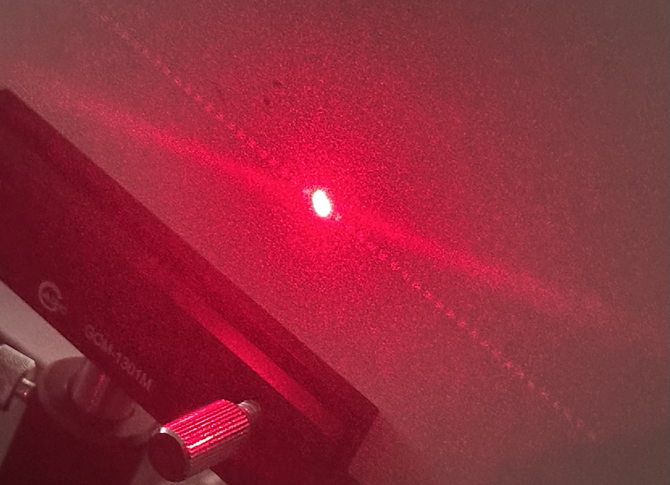
\includegraphics[width=\linewidth]{imgs/s2.png}
            \captionof{figure}{S2}
        \end{minipage} & 
        \begin{minipage}[t]{0.3\textwidth}
            \centering
            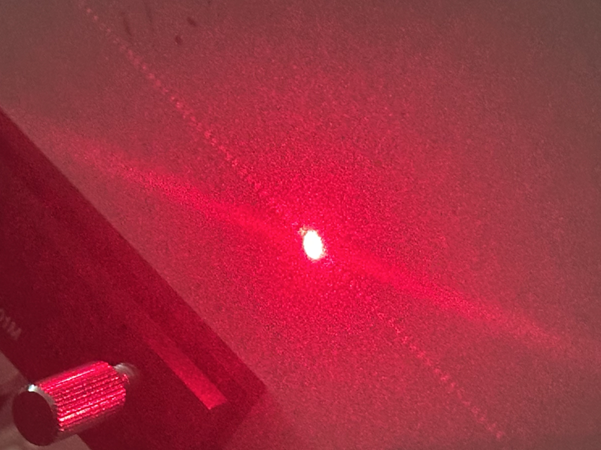
\includegraphics[width=\linewidth]{imgs/s3.png}
            \captionof{figure}{S3}
        \end{minipage} \\
        \begin{minipage}[t]{0.3\textwidth}
            \centering
            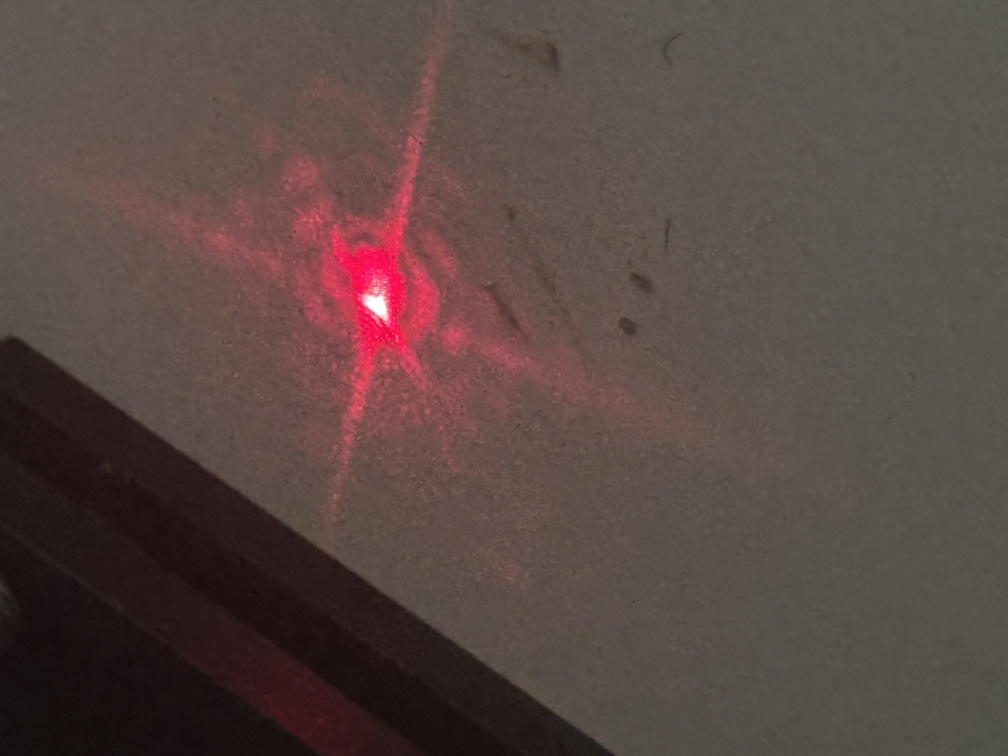
\includegraphics[width=\linewidth]{imgs/xk1.png}
            \captionof{figure}{XK1}
        \end{minipage} & 
        \begin{minipage}[t]{0.3\textwidth}
            \centering
            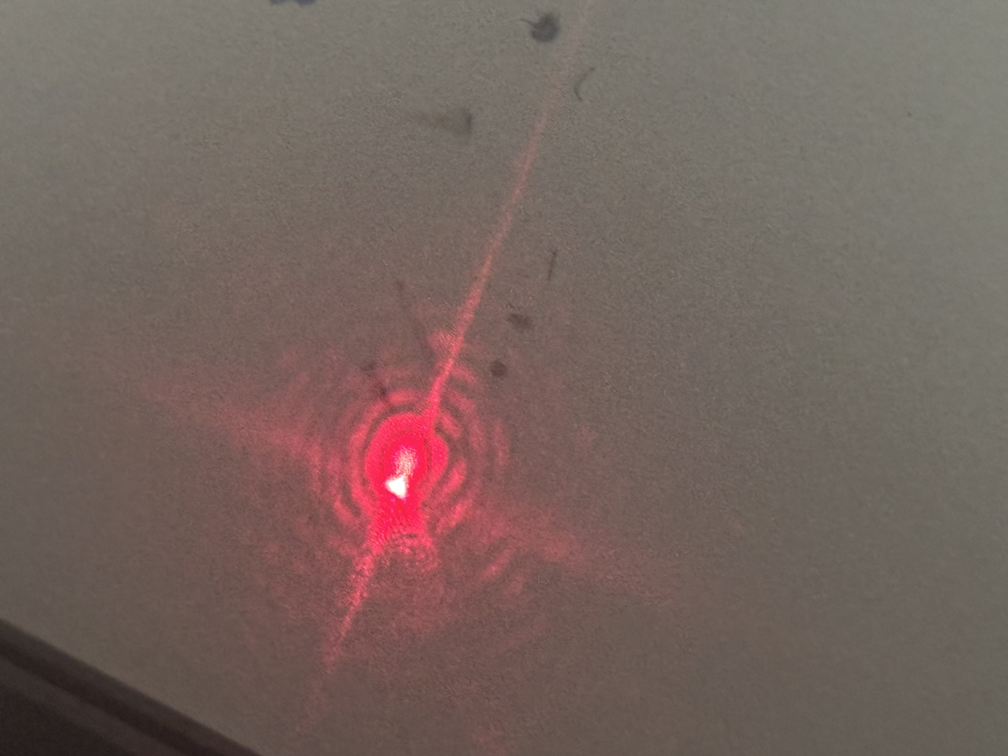
\includegraphics[width=\linewidth]{imgs/xk2.png}
            \captionof{figure}{XK2}
        \end{minipage} & 
        \begin{minipage}[t]{0.3\textwidth}
            \centering
            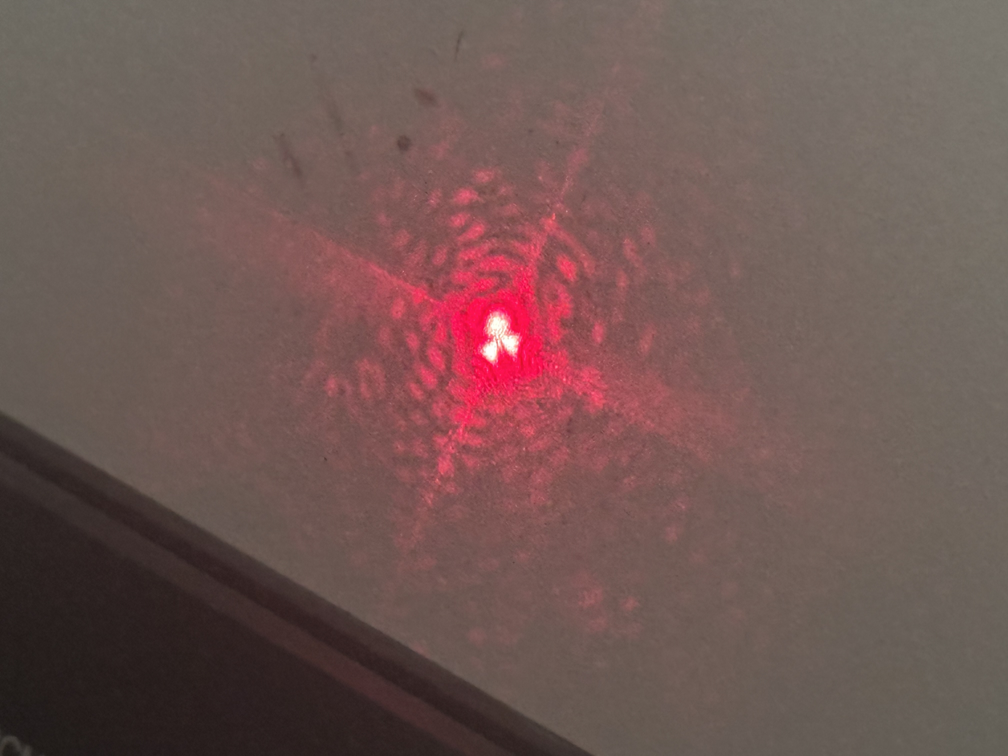
\includegraphics[width=\linewidth]{imgs/xk3.png}
            \captionof{figure}{XK3}
        \end{minipage} \\
        \begin{minipage}[t]{0.3\textwidth}
            \centering
            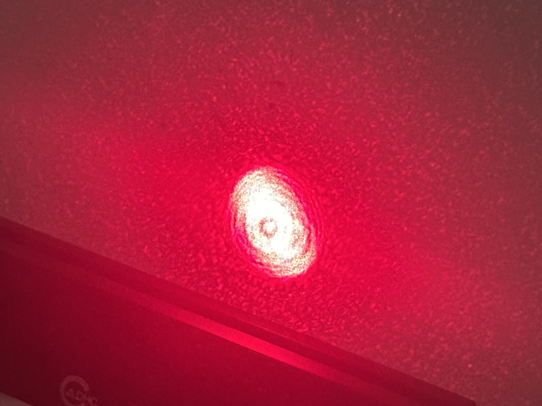
\includegraphics[width=\linewidth]{imgs/xp1.png}
            \captionof{figure}{XP1}
        \end{minipage} & 
        \begin{minipage}[t]{0.3\textwidth}
            \centering
            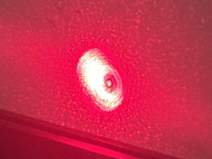
\includegraphics[width=\linewidth]{imgs/xp2.png}
            \captionof{figure}{XP2}
        \end{minipage} & 
        \begin{minipage}[t]{0.3\textwidth}
            \centering
            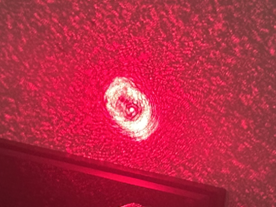
\includegraphics[width=\linewidth]{imgs/xp3.png}
            \captionof{figure}{XP3}
        \end{minipage} \\
        \hline
    \end{tabular}
    \caption{分划板1衍射图像}
\end{table}
\newpage
对于分划板2, 我们观察到了如下的衍射图像, 其中各种光栅的参数同样可参考实验仪器部分的表格. 
\begin{table}[h!]
    \centering
    \begin{tabular}{|ccc|}
        \hline
        \begin{minipage}[t]{0.3\textwidth}
            \centering
            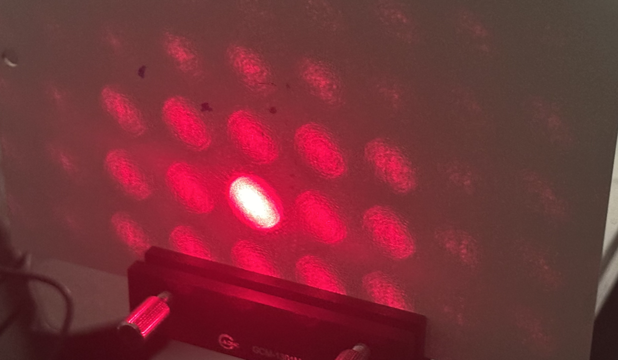
\includegraphics[width=\linewidth]{imgs/gs1.png}
            \captionof{figure}{GS1}
        \end{minipage} & 
        \begin{minipage}[t]{0.3\textwidth}
            \centering
            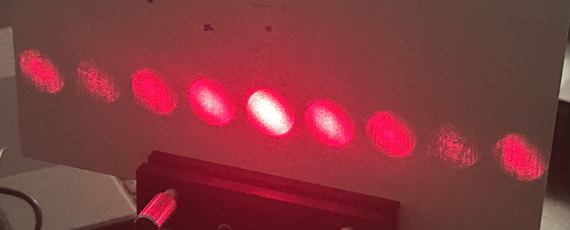
\includegraphics[width=\linewidth]{imgs/gs2.png}
            \captionof{figure}{GS2}
        \end{minipage} & 
        \begin{minipage}[t]{0.3\textwidth}
            \centering
            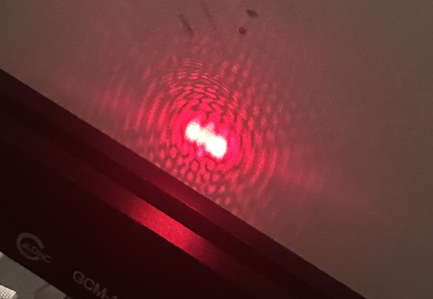
\includegraphics[width=\linewidth]{imgs/sk1.png}
            \captionof{figure}{SK1}
        \end{minipage} \\
        \begin{minipage}[t]{0.3\textwidth}
            \centering
            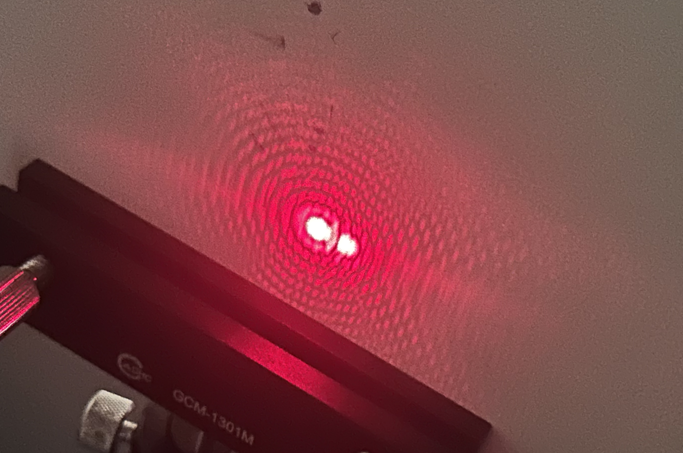
\includegraphics[width=\linewidth]{imgs/sk2.png}
            \captionof{figure}{SK2}
        \end{minipage} & 
        \begin{minipage}[t]{0.3\textwidth}
            \centering
            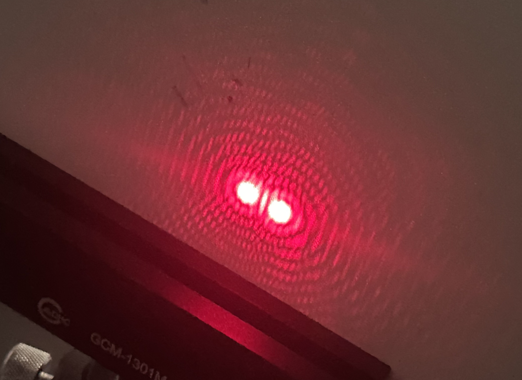
\includegraphics[width=\linewidth]{imgs/sk3.png}
            \captionof{figure}{SK3}
        \end{minipage} & 
        \begin{minipage}[t]{0.3\textwidth}
            \centering
            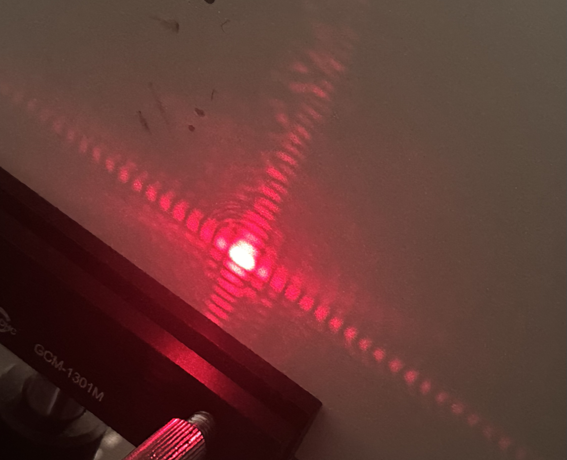
\includegraphics[width=\linewidth]{imgs/jk.png}
            \captionof{figure}{JK}
        \end{minipage} \\
        \begin{minipage}[t]{0.3\textwidth}
            \centering
            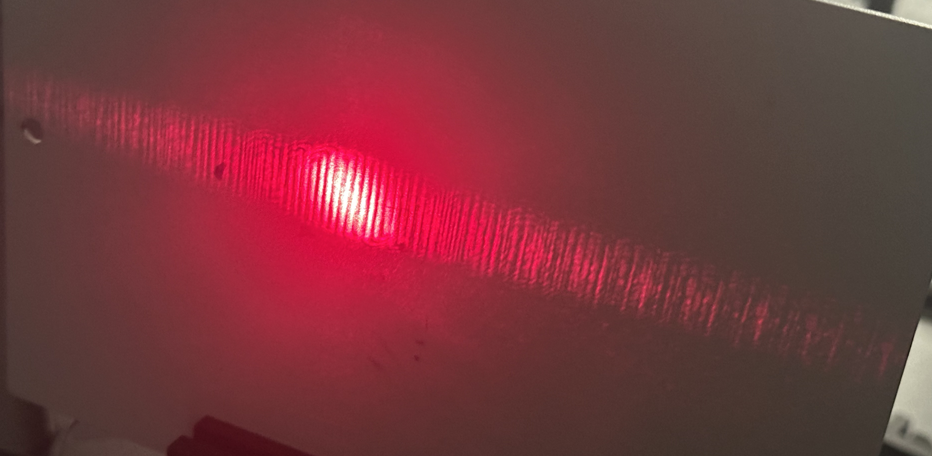
\includegraphics[width=\linewidth]{imgs/duof2.png}
            \captionof{figure}{DF2}
        \end{minipage} & 
        \begin{minipage}[t]{0.3\textwidth}
            \centering
            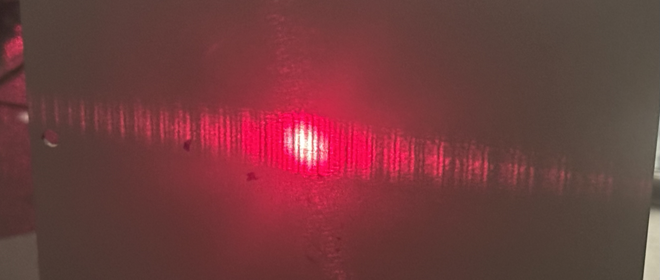
\includegraphics[width=\linewidth]{imgs/duof1.png}
            \captionof{figure}{DF1}
        \end{minipage} & 
        \begin{minipage}[t]{0.3\textwidth}
            \centering
            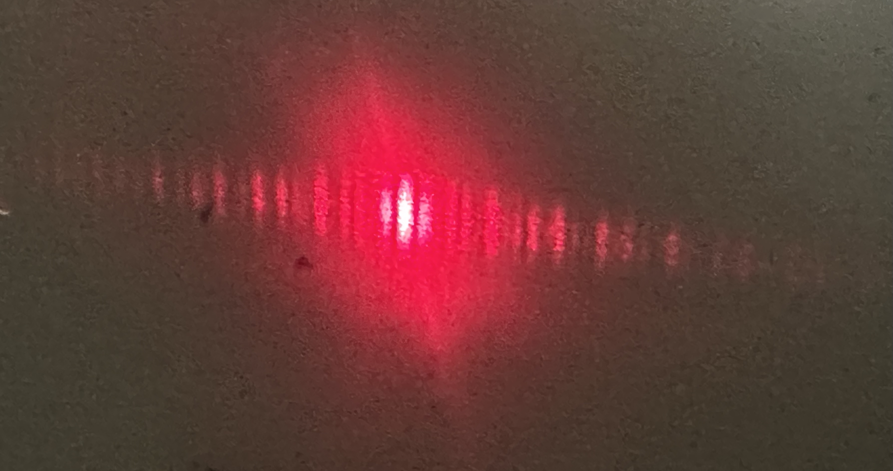
\includegraphics[width=\linewidth]{imgs/sf3.png}
            \captionof{figure}{SF3}
        \end{minipage} \\
        \begin{minipage}[t]{0.3\textwidth}
            \centering
            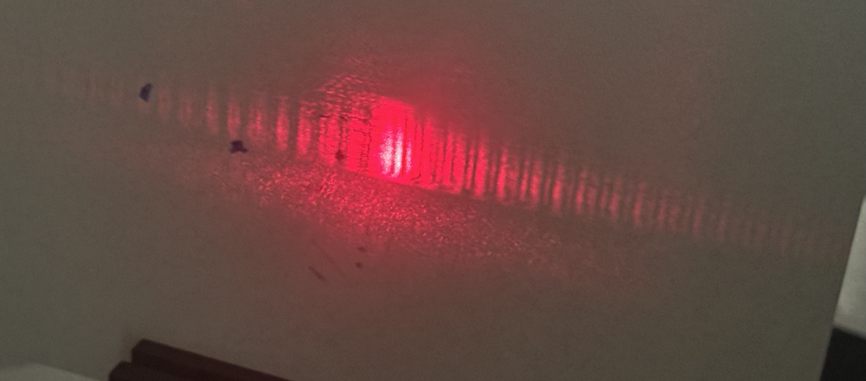
\includegraphics[width=\linewidth]{imgs/sf2.png}
            \captionof{figure}{SF2}
        \end{minipage} & 
        \begin{minipage}[t]{0.3\textwidth}
            \centering
            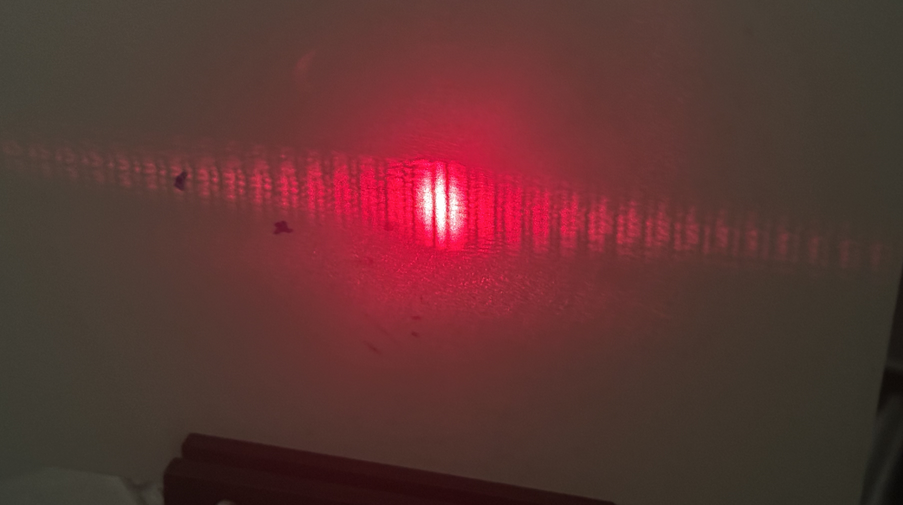
\includegraphics[width=\linewidth]{imgs/sf1.png}
            \captionof{figure}{SF1}
        \end{minipage} & 
        \begin{minipage}[t]{0.3\textwidth}
            \centering
            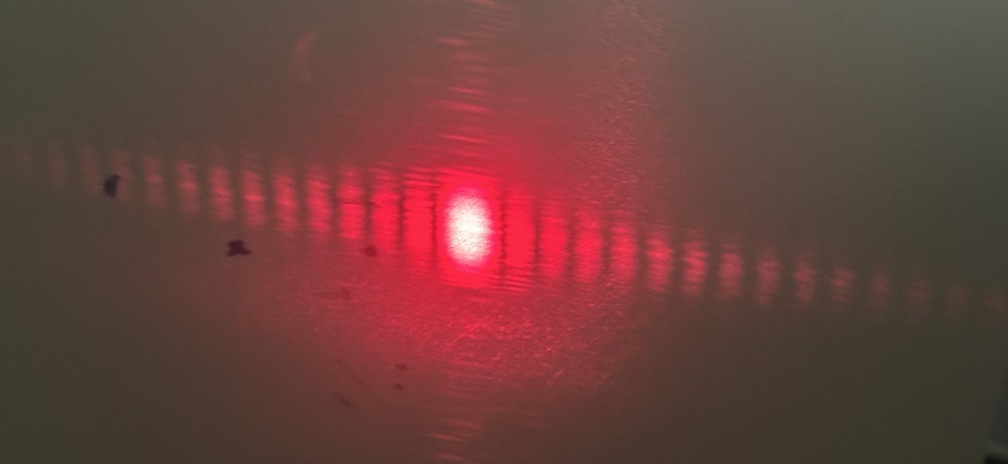
\includegraphics[width=\linewidth]{imgs/danf1.png}
            \captionof{figure}{DF1}
        \end{minipage} \\
        \hline
    \end{tabular}
    \caption{分划板2衍射图像}
\end{table}
\subsection{光栅衍射测量光栅常数实验}
\subsubsection{光路布置调节}
\begin{figure}[H]
    \centering
    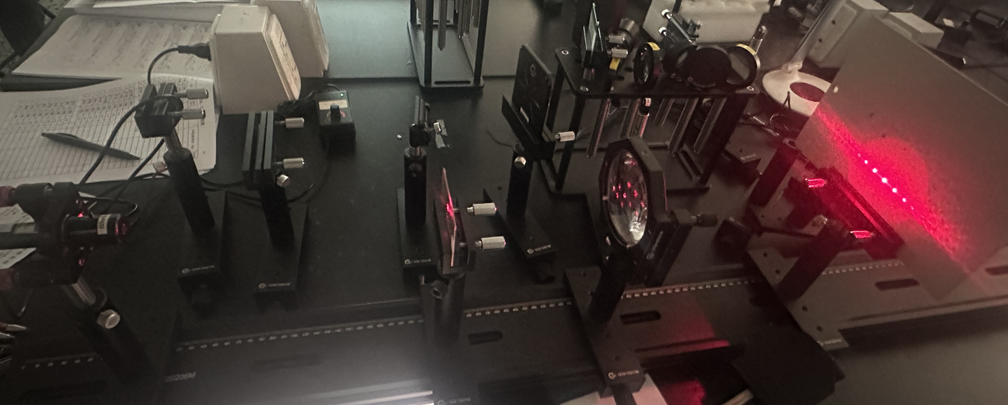
\includegraphics[width=0.6\textwidth]{imgs/测量光栅常数光路.png}
    \caption{光栅衍射测量光栅常数实验光路}
\end{figure}
\subsubsection{测量结果和计算}
我们测得光栅到光屏的距离为$x = 39\mathrm{cm}$, 光屏上相邻两个级大的距离为$x = 2.6\mathrm{cm}$, 则我们可以计算出
\[
\sin \theta = \dfrac{y}{\sqrt{y^2 + x^2} } \implies d = \dfrac{\lambda}{\sin \theta}
\] 
我们使用的激光的波长为$\lambda = 650\mathrm{nm}$, 从而我们可以计算得光栅常数为 $f = \dfrac{1}{d} = 102.337$
\subsection{光栅光谱仪测光谱实验}
我们分别对白色LED灯, 红色激光灯, 显示绿色的平板屏幕和日光进行了测量, 测量结果如下

\begin{table}[H]
    \centering
    \begin{tabular}{|cccc|}
        \hline
        \begin{minipage}[t]{0.2\textwidth}
            \centering
            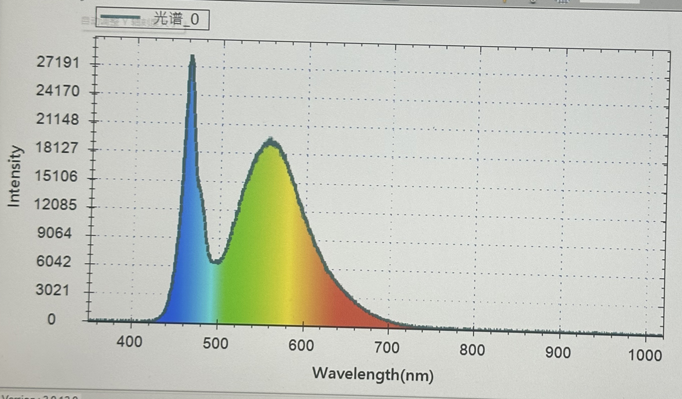
\includegraphics[width=\linewidth]{imgs/光谱仪1.png}
            \captionof{figure}{LED白光}
        \end{minipage} & 
        \begin{minipage}[t]{0.2\textwidth}
            \centering
            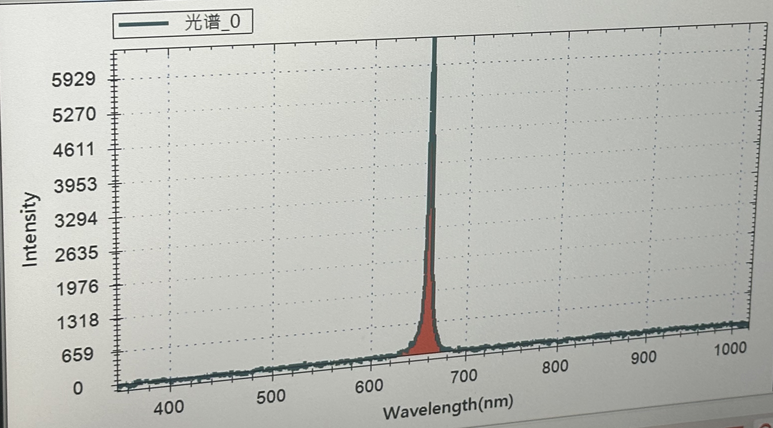
\includegraphics[width=\linewidth]{imgs/光谱仪2.png}
            \captionof{figure}{激光器红光}
        \end{minipage} &
        \begin{minipage}[t]{0.2\textwidth}
            \centering
            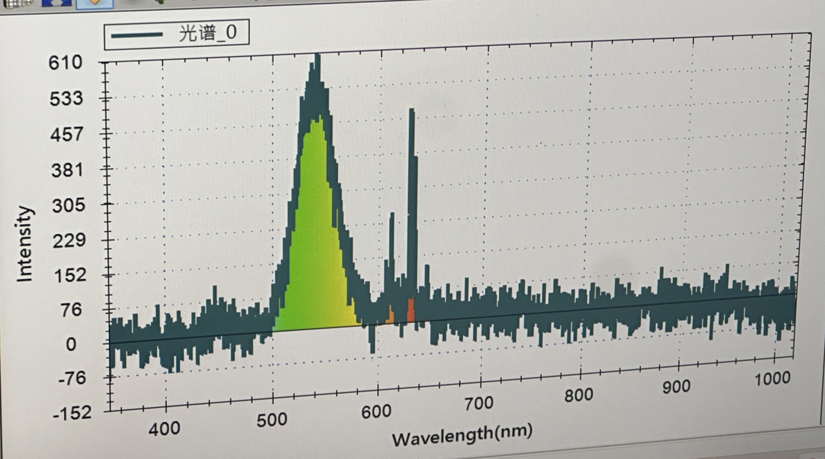
\includegraphics[width=\linewidth]{imgs/光谱仪3.png}
            \captionof{figure}{平板绿光}
        \end{minipage} & 
        \begin{minipage}[t]{0.2\textwidth}
            \centering
            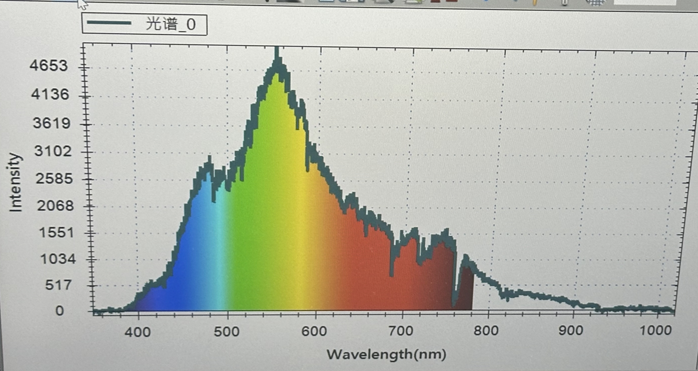
\includegraphics[width=\linewidth]{imgs/光谱仪4.png}
            \captionof{figure}{自然日光}
        \end{minipage} \\
        \hline
    \end{tabular}
    \caption{光栅光谱仪测光谱实验}
\end{table}

\section{实验总结与思考}

\subsection{实验总结}

本次实验主要通过搭建光路观测在光屏上出现的图像来验证物理规律, 过程中需要大量的观察以及图像记录. 在阿贝成像实验中, 我们通过改变滤波器的方向来实现对光不同方向的滤波. 具体而言, 滤波器的放置方向与最终出现的条纹方向垂直, 说明了滤波器保留了其放置方向的信息, 滤去了垂直方向的信息. 实验中需要不断对光源进行调整以及对各种仪器的调整来保证光垂直的打在光屏上, 确保最后得到的图像清晰并且符合预期出现的结果. 

光学4F系统成像实验在阿贝成像实验的基础上进行了一定的改进, 成像更加清晰, 并且得到的是与物体等大反向的像, 其它结果与阿贝成像实验类似

假彩色编码实验主要是通过调整$\theta$调制滤波器来实现对天安门城楼图像不同区域的上色, 过程中需要精细的调整滤波器的位置来保证频谱上的各种颜色被准确地过滤

光栅光谱仪实验中, 我们通过观察夫琅和费衍射的图像来验证光栅的参数, 建议在使用分划板前先对其进行擦拭, 以保证成像效果. 在测量光栅常数时, 我们需要测量光栅到光屏的距禛以及相邻两个级大的距离, 通过这两个数据我们可以计算出光栅的常数. 在测量光谱时, 我们通过光栅光谱仪测量了白色LED灯, 红色激光灯, 显示绿色的平板屏幕和日光的光谱, 通过观察光谱的形状我们可以得到不同光源的光谱特征. 

\subsection{实验思考}
讲义中参考的距离和实际的最佳距离仍有一定的差距, 不应该完全按照讲义上的数据设置光路, 最好的办法还是通过实践得到的结果来进行调整. 

由于实验环境较暗, 当使用手机拍照时, 由于手机自动开启夜景模式自动曝光时间过长, 而且在此过程中会不可避免地手抖, 这就是导致拍摄的图像中的条纹不够清晰. 因此在拍摄图像时要注意拍摄的仪器, 同时要保证相机的稳定性

对于分划板中不同口径的光栅, 我们可以通过观察其衍射图像来得到不同光栅的参数, 这是一种非常有效的方法, 但是在实际拍摄过程中由于拍摄的角度和距离的不同, 所呈现的图像并不能很好地反映光栅的不同参数, 因此需要以实际测量结果为准

\section{思考题}
\subsection{阿贝成像相关}
\subsubsection{ 阿贝成像中,当“缝”与光栅方向夹角 45 度放置滤波时,会有何效果?}
得到的像中间充满斜条纹, 且斜条纹的方向和滤波器缝的方向垂直
\subsubsection{前面实验中,我们使用低通滤波(仅让 0 级斑通过)实现了光栅格子信息的消除;如何做个高通滤波的例子?应该如何实现和它的效果是什么?}
在频谱平面上放置一个不透光的小圆盘, 其中心正好位于零级斑的位置. 这个小圆盘就起到了高通滤波器的作用. 就效果而言,高通滤波器滤除了低频成分, 使得图像的边缘部分变得更加突出, 有利于边缘检测和特征提取. 
\subsection{观察 4F 系统成像与阿贝成像时单透镜成像的区别是什么?}
4F系统的保真性、稳定性更好的, 成像更加清晰, 与物体等大, 且是倒立的
\subsection{假彩色编码实验中使用的天安门城楼光栅本身中的城楼的窗户和门洞都是透光的,但是为什么经过所提供的假着色滤波处理后所成的像中这些窗户和门洞是黑色的?有方法验证你的解释吗?}
因为$\theta$调制滤波器的中间是不透光的, 所以如果通过$\theta$调制滤波器中间部分的光正好是对应天安门城楼光栅的城楼的窗户和门洞部分的光, 这些光在通过$\theta$滤波器时由于被不透光的部分遮挡, 所以滤波处理后窗户和门洞是黑色的. 

验证方法: 制作一个中间透光的$\theta$调制滤波器, 然后观察成像效果, 应该会发现窗户和门洞是透明的
\subsection{从夫琅和费衍射演示实验得到哪些规律?}
主要能得到如下规律:
\begin{enumerate}
    \item \textbf{中央明纹最宽, 亮度最大} \\
    无论是单缝衍射还是多缝衍射, 中央明纹总是最宽的, 亮度也最高. 这与光的干涉原理密切相关, 中央明纹处各波光程差为零, 发生加强干涉. 

    \item \textbf{明暗条纹交替分布} \\
    在中央明纹两侧, 明暗条纹交替出现. 

    \item \textbf{条纹宽度与缝宽的关系} \\
    \textbf{单缝衍射: } 缝宽越窄, 衍射现象越明显, 中央明纹越宽, 两侧暗纹之间的距离越大.  \\
    \textbf{多缝衍射: } 缝宽不变时, 缝数越多, 主极大越尖锐, 次极大越弱, 衍射图样中明暗条纹的对比度越大. 
\end{enumerate}
\end{document}
